\newcounter{test}
\newcommand\AdvecTitle{%
  \frametitle{\refstepcounter{test} Advection equation~\thetest}}
\resetcounteronoverlays{test}


\begin{frame}[fragile]
%\frametitle{Advection equation}
\AdvecTitle
\begin{itemize}
\item Linear advection equation.
      \begin{fleqn}
      \begin{equation}
      \frac{\partial u}{\partial t} + c \frac{\partial u}{\partial x} = 0, \qquad
      c \geq 0
      \label{eq:advection}
      \end{equation}
      
      \begin{equation}
      u\left(x,0\right)=u_0 \nonumber
      \label{eq:advection}
      \end{equation}
      \end{fleqn}
\end{itemize}
\end{frame}

\begin{frame}[fragile]
%\frametitle{Advection equation}
\AdvecTitle
\begin{itemize}
\item Initial condition and analytical solution at t=2.0000.
	  \begin{fleqn}
      \begin{equation}
      u_0 = \begin{cases} 1.0 \qquad 2.0 \leqslant x \leqslant 4.0 \\ 0.0 \qquad other \end{cases} \nonumber
      \end{equation}
      \end{fleqn} 

\begin{figure}
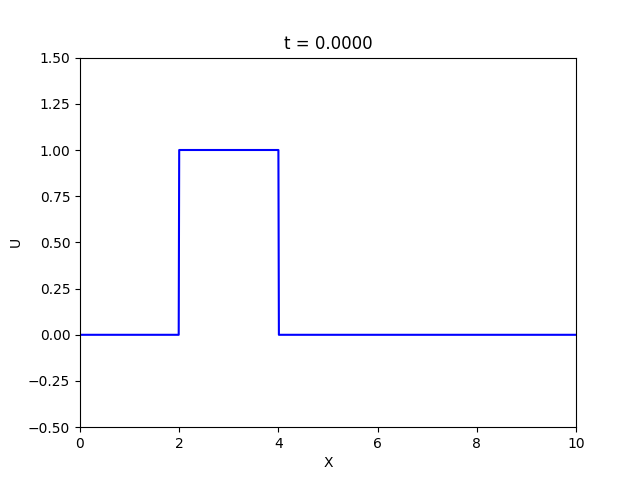
\includegraphics[width=0.5\textwidth, height=0.25\textwidth]{./image/init.png}%
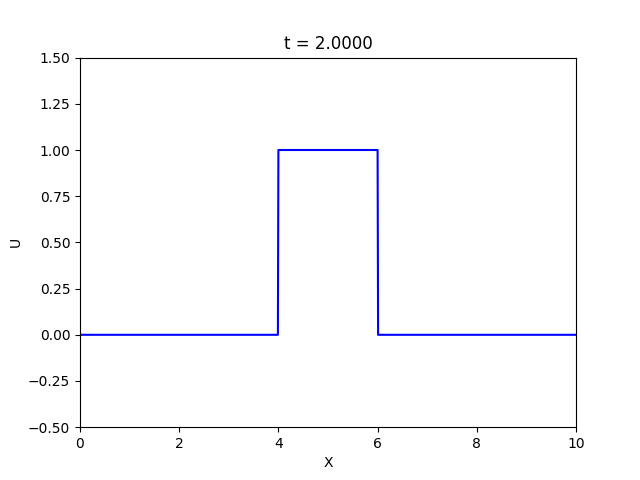
\includegraphics[width=0.5\textwidth, height=0.25\textwidth]{./image/final.png}
\caption{Left is at t=0.0000 and right is at t=2.0000}
\end{figure}

\end{itemize}
\end{frame}


\begin{frame}[fragile]
\AdvecTitle
\begin{itemize}
\item Sample of upwind discretization in Python.
\lstinputlisting[language=Python, firstline=1, lastline=2]{./codes/upwind.py}
\lstinputlisting[language=Python, firstline=27, lastline=36]{./codes/upwind.py}

\end{itemize}

\end{frame}